\chapter{Implementation}\label{chap:implementation}

Since we designed MPDTLS as an extension for DTLS, it was logical not to implement it from scratch but to start from an existing implementation of DTLS. Multiple libraries implement the latest version \footnote{\url{https://en.wikipedia.org/wiki/Datagram_Transport_Layer_Security\#Implementations}}, but we chose wolfSSL \cite{wolfssl} (previously CyaSSL) as our starting point.

The choice was driven by the following criteria :
\begin{itemize}
\item Code readability
\item Documentation
\item Existing examples
\item Library size
\end{itemize}

Unlike OpenSSL, wolfSSL contains a reduced number of files to handle SSL/TLS and DTLS. The objective of this library is to be as light as possible to allow integration in embedded systems. As stated in their official website \footnote{\url{http://www.yassl.com/yaSSL/Home.html}}, the library is up to 20 times smaller than OpenSSL.

Documentation and working examples are provided to help its use. For all these reasons, we chose to work with wolfSSL. In the following sections, we are going to explain how this library works, how we integrate our additions to DTLS and the various issues we faced during the implementation.

\section{Packet reception}\label{sec:packet-reception}
The first step is to make the library recognizes the new packets and handles them correctly, like issuing a \texttt{FeedbackAck} upon reception of a \texttt{Feedback}. This part is quite easy once the internal flow followed by the received packets is understood. The flow we are going to explain is pictured in the Figure \ref{fig:readdiag}. The call related to mutex are not part of the original wolfSSL code and are explained in the Section \ref{sec:threadsafe}.

First of all, it is important to recall wolfSSL is a library and thus does not have any existence outside the call made in the client code.

To receive packets, an application must call the \texttt{wolfSSL\_read(WOLFSSL*,void*,int)} function once all the library is correctly set up. When this function is call, the process enters the library, dives into the \texttt{ReceiveData} and \texttt{ProcessReply} functions and will eventually make a blocking call into the \texttt{CBIORecv} macro\footnote{The low-level mechanisms to read and write on sockets are indeed encapsulated into macros selected following the compilation or configuration flags. This provides to the library some cross-platform aspects.} to listen on the socket. When a new packet arrives, the process is woke up and it copies the packet into an internal buffer. Once the copy is made and the pointers correctly set, the process can treat the packet.

\begin{figure}[!hp]
\centering
\begin{sequencediagram}
\centering
\newthread[blue]{r}{wolfSSL\_read}
\newinst{rd}{ReceiveData}
\newinst{pr}{ProcessReply}
\newinst{gid}{GetInputData}
\newinst{rc}{Receive}
\newinst{grh}{GetRecordHeader}
%\newinst{do}{Do\textit{Type}}

\begin{call}{r}{MutexLock}{r}{}
\end{call}
\begin{call}{r}{}{rd}{}
    \begin{sdblock}{while}{no content in \texttt{clearOutputBuffer}}
        \begin{call}{rd}{}{pr}{}
            \begin{call}{pr}{}{gid}{}
                \begin{call}{gid}{}{rc}{}
                    \begin{call}{rc}{MutexUnlock}{rc}{}
                    \end{call}
                    \begin{call}{rc}{\texttt{CBIORecv}}{rc}{}
                        \postlevel
                    \end{call}
                    \begin{call}{rc}{MutexLock}{rc}{}
                    \end{call}
                \end{call}
            \end{call}
            \begin{call}{pr}{}{grh}{\shortstack{\textit{ContentType}\\Length}}
                \postlevel
            \end{call}
            \begin{sdblock}{switch}{on \textit{ContentType}}
                \begin{call}{pr}{Do\textit{ContentType}}{pr}{}
                    \postlevel
                \end{call}
            \end{sdblock}
        \end{call}
    \end{sdblock}
\end{call}
\postlevel
\begin{call}{r}{MutexUnlock}{r}{}
\end{call}
\end{sequencediagram}
\caption{Major functions called on \texttt{wolfSSL\_read()}\label{fig:readdiag}}
\end{figure}


First, it reads the \texttt{RecordLayer} header, containing the length of the packet and the type of the Record. The latter can be one of the \texttt{ContentType} value defined in the RFC. During this verification, it also define, based on the \texttt{ContentType} value, if the packet is encrypted and therefore needs to be deciphered before handling it.

Then, after the decryption of the packet if it was needed, the packet is dispatched to the handling function corresponding to the Record type. These functions are called following the pattern "\texttt{Do}\textit{TypeName}" (e.g. \textit{DoApplicationData} to handle AppData packets). For the sake of clarity, these two steps (decryption and all possible \texttt{Do}functions) are not represented on the Figure \ref{fig:readdiag}.


In the case of the original implementation of wolfSSL, the only Record type that could be encountered at this point was AppData. The function \textit{DoApplicationData} does some treatments on the packet like verifying the MAC or decompressing the packet if needed and finally copies the clear content of the packet into a specific buffer called \texttt{clearOutputBuffer}. Then, if the input buffer has been completely consumed, the process comes back to the function \texttt{ReceiveData}. This function copies the content of \texttt{clearOutputBuffer} to the application buffer passed in argument of \texttt{wolfSSL\_read}, giving to the client application the content of the received packet. The library will then exit and give the control back to the calling code.

\subsection{Adding new types}

Adding the recognition of a new type is done in two steps, after the defininion of all the needed declarations in the header file: we start by adding the type in the switch of the \texttt{GetRecordHeader} function. We can also add indication about the packet type, such as if the content is ciphered or not. Then, we need to add a new case for the type in the switch statement of the \texttt{ProcessReply} function, in which we prepare and make the call to a new, dedicated function \texttt{Do\textit{TypeName}}.

Now that library recognizes the new type and call the appropriate \texttt{Do}function, we can implement the latter with the intended behavior. In our case, we use the \texttt{DoApplicationData} as a base for the implementation of all the \textit{Do}function of protocol-level packet types (e.g. \texttt{Feedback}, \texttt{WantConnect}\dots). It is the easiest solution to get ciphering and authentication of the packets.But it is important to not let these packets leave the library and be delivered to the application. To achieve this, we move the pointer marking the end of the \texttt{clearOutputBuffer} before the beginning of the current packet, once we have finished the treatment of the packet.

\section{Packet emission}

The packets emission is even simpler, as we don't have to wait for some event, we trigger it. So, in wolfSSL, an application can send packets by the use of the \texttt{wolfSSL\_write(WOLFSSL*, void*, int)} function. As shown in the Figure \ref{fig:writediag}, the process then enters in \texttt{SendData}, which is responsible of all the authentication and encryption stuff, in the original code of the library. We moved the code handling the MAC and encryption in a new function \texttt{SendPacket}, allowing us to use the encryption not only for the Application Data packets but also for our protocol-level packets. As for the receiving functions, we created a set of \texttt{Send\textit{TypeName}} functions, in charge of building the corresponding packets before sending them. All these methods end by calling \texttt{SendPacket} which will then call \texttt{SendBuffered}. \texttt{SendBuffered} is the last function in the library before leaving the control to the concrete sending macro \texttt{CBIOSend}, and this is the place we choose to put our scheduling mechanism. The socket to use is thus chosen at the beginning of \texttt{SendBuffered}, just before the call to the sending function.

\begin{figure}[!h]
\centering
\begin{sequencediagram}
\centering
\newthread[blue]{w}{wolfSSL\_write}
\newinst{sd}{SendData}
\newinst{sp}{SendPacket}
\newinst{bm}{BuildMessage}
\newinst{sb}{SendBuffered}
%\newinst{do}{Do\textit{Type}}

\begin{call}{w}{MutexLock}{w}{}
\end{call}
\begin{call}{w}{}{sd}{}
        \begin{call}{sd}{}{sp}{}
            \begin{call}{sp}{}{bm}{}
                \begin{call}{bm}{AddRecordHeader}{bm}{}
                \end{call}
                \begin{call}{bm}{Encrypt}{bm}{}
                \end{call}
                \begin{call}{bm}{HashOutput}{bm}{}
                \end{call}
            \end{call}
            \begin{call}{sp}{}{sb}{}
                \begin{call}{sb}{\texttt{CBIOSend}}{sb}{}
                    \postlevel
                \end{call}
            \end{call}
        \end{call}
\end{call}
\begin{call}{w}{MutexUnlock}{w}{}
\end{call}
\end{sequencediagram}
\caption{Major functions called on \texttt{wolfSSL\_write()}\label{fig:writediag}}
\end{figure}

\section{Thread-safety}\label{sec:threadsafe}

A major drawback of living at the application-level as a library is that you are really dependent of the application that uses you. For instance, all protocol-level packets need responses to ensure the reception, since DTLS is not reliable. But, to trigger the internal mechanisms explained in the previous sections, the library must be in a listening state, constantly. If an application needs to send some packets, which seems to be a normal use case of the library, it will need to use threads to read and write simultaneously. For this reason, we need to be sure that using the library in such way will not cause trouble. As the library uses a lot of internal buffers when it reads or writes, and that our treatments of protocol-level packets involves packets emission during packets reading, we considered the whole library code as a critical section, with a notable exception for the blocking call in the \texttt{Receive} function\footnote{As a call to \texttt{select} is blocking, it prevents the application to write packets when the other thread waits for incoming packets, which would add an extra undesirable overhead.}.

Thus, as with every critical section that you want to protect, we added a mutex to lock when entering either \texttt{wolfSSL\_read} or \texttt{wolfSSL\_write} and unlocked just before leaving these functions. This mutex is also unlock just before the blocking call to select and relock right after the select returns.

\subsection{What about processes ?}

Using processes instead of the threads is another solution, but either processes have to use different session credentials or have to share memory to use the same session object. One could propose to simply duplicate the session either through the session resuming or via copy-on-write session mechanisms, but just having the same session credentials is not sufficient to the library to correctly work. As we use statistics to choose the best path to send new packets, the session object must be completely in sync between the processes, with all the risks of memory corruption due to the simultaneous accesses. We finally end up in the same situation as with the threads.

For the sake of simplicity, we recommend thus to simply use threads, as we made our best to get a thread-safe library.

\section{Managing timed (re)transmissions}

Since we work on a library, we may not to whatever we want. For instance, it is a bad design choice to do interruptions in the library. And this is a problem as we have to handle timeouts and retransmissions for the control-level packets. Note that by timeout we mean either that the packet has not been acknowledged by the other host or that the packet must be sent periodically and the last sending occurred too long ago.

We thus had to use other ways to detect that a packet needs retransmission. By checking actively after each packet sent, we can overcome the need of interruption mechanism. This check is implemented with the addition of the call to the \texttt{CheckTimeouts} function, just before the return of \texttt{SendBuffered}. This function verifies that neither \texttt{Heartbeat} message nor \texttt{CIM} needs (re)transmission. To know which packet needs to be retransmitted because it is in timeout state, we use two possible criteria. First, we base the timeout on the time elapsed since the last packet was sent. Second, we use as trigger the number of packets sent since the last packet of the considered type was sent.

\subsection{Timeouts}

With this strategy, we are guaranteed to retransmit the packet within a delimited time window, given that other packets are sent since we check the timeouts only at this moment. The implementation of this part is quite simple as we just need to store the current time when we send the packet. The verification then consists in simply comparing the difference between the stored time value and the current time with a defined timeout offset.

As the protocol does not give any guarantee about the delivery of \texttt{ApplicationData} packet but requires that \texttt{Heartbeat} and \texttt{CIM} are transmitted reliably, we use this strategy to ensure the retransmission. Also, the \texttt{Heartbeat} messages being sent periodically, this mechanism can also answer the need.

Concerning our implementation, the timeval for the \texttt{CIM} is stored in the general structure of wolfSSL, while each sub-flow stores the timeval for its \texttt{Heartbeat}, since each sub-flow manages its own \texttt{Hearbeat} exchange.

\subsection{Packets count}

If the previous strategy guaranteed us some time bounds on the trigger, the "packet-count" strategy allows us to have a more adaptive transmission in regards of the actual traffic. As the feedback primary purpose is directly related to the amount of traffic on a flow, we decided to use this strategy for the \texttt{Feedback} packets, both for the transmission and retransmission in case of missing acknowledgement.

While the design does not require that the exchange of \texttt{Feedback} reports is reliable (see Section \ref{sec:feedbackReport}), we chose to reduce the number of packet to aggregate before sending feedback in case of incremental feedback. That is, when the \texttt{Feedback} or \texttt{FeedbackAck} is lost. The purpose of this reduction is to increase the rate of \texttt{Feedback} message and thus speed up the acknowledgement of feedback and free the memory used to store the cache. The details of this will be explained in the Section \ref{sec:impl-stats}.

\section{Multipath integration}

The multipath part of the implementation requires some modifications at some strategic points: selection of a flow to send a packet, reception from all the sub-flows simultaneously,\dots We also need to store a few structures in memory to keep sub-flows state and statistics. This section aims to cover all these modifications, that make multipath possible in wolfSSL.

\subsection{Memory structures}

To be able to use multipath, we needed to store some information in the memory, like the addresses the application wants to advertise, the addresses of the remote host, the created sub-flows and their statistics, the flows waiting for confirmation and the sockets opened to reserve port number but not actively used in a sub-flow. We have implemented helper functions to handle these structures easily, such as inserting new elements, removing element by index or with some criteria and searching for elements. These functions take care of reallocating the memory correctly, to keep the memory footprint as low as possible.

\addtypes{struct,timeval,byte,uint,word16,MessageState,sockaddr_storage,uint}

\begin{lstlisting}[caption=Structure storing addresses]
typedef struct MPDTLS_ADDRS {
    struct sockaddr_storage* addrs;    /* Contains all the available addresses
                                          for MPDTLS (both IPV4 or IPV6) */
    int                      nbrAddrs; /* Number of available addresses */
} MPDTLS_ADDRS;
\end{lstlisting}

In our implementation, we have added two \texttt{MPDTLS\_ADDRS} structures in the general \texttt{WOLFSSL} \textit{session object} and one in the \texttt{WOLFSSL\_CTX} \textit{context object}.

The first structure \texttt{mpdtls\_host} contains the addresses advertised by the host. An application can insert new address into this list by two ways. First, it can call the \texttt{wolfSSL\_mpdtls\_new\_addr (WOLFSSL*, const char*)} function, with the session object and an address as a string, under either IPv4, IPv6 or DNS format, as arguments. The other way is \texttt{wolfSSL\_mpdtls\_new\_addr\_CTX (WOLFSSL\_CTX*, const char*)}. This contextual variant adds the address into the context object rather than in the session object. All the sessions created from this context will inherit its host addresses. To ensure that this list of registered addresses is correctly synchronised, a \texttt{CIM} is issued either each time a new address is added or just after the handshake of a session inheriting addresses from its context.

The second structure \texttt{mpdtls\_remote} stores the addresses advertised by the other host. It is updated only upon reception of a \texttt{ChangeInterfaceMessage} and is used to know which sub-flows can be created.

\begin{lstlisting}[caption=Structure containing inactive socket,label=lst:sockpool]
typedef struct MPDTLS_SOCKS {
    int* socks;    /* Contains all the available sockets for MPDTLS */
    int  nbrSocks; /* Number of available sockets */
} MPDTLS_SOCKS;
\end{lstlisting}

However, from the Section \ref{sec:advertise} and more specifically the Listing \ref{lst:cimformat}, we can see that each address advertised must also mention the port reachable for the flow. As the flow does not already exist, the port is not already known at the time of advertisement. To determine this port, we let the OS attribute one to the application simply by opening a socket. We then retrieve the port number and register it in the \texttt{MPDTLS\_ADDRS} structure. But, if we delete the socket right after, there no guarantee that the port number that we got will not be reassigned, and thus would become unavailable. To avoid that, we store the created socket in a \texttt{MPDTLS\_SOCKS} structure (Listing \ref{lst:sockpool}). When we finally create a flow with the address corresponding to a socket of this pool, we reuse it instead of creatint a new socket. In this way, we keep the amount of open socket low while keeping the advertised port number safe.

\begin{lstlisting}[caption=Structures handling flows, label=lst:flow]
typedef struct MPDTLS_FLOW_HEARTBEAT {
    struct timeval last_heartbeat;         /* last timestamp */
    byte           response_rcvd;          /* whether or not we have received
                                              a response to our heartbeat */
    uint           rtx_threshold;          /* the retransmission threshold
                                              will be higher if no response */
    byte*          heartbeatPayload;       /* heartbeat payload */
    word16         heartbeatPayloadLength; /* length */
    MessageState   heartbeatState;         /* avoid multiple heartbeat tx */
} MPDTLS_FLOW_HEARTBEAT;

typedef struct MPDTLS_FLOW {
    struct sockaddr_storage host;           /* flow determined by the host */
    struct sockaddr_storage remote;         /* & remote sockaddr (ip+port) */
    int                     sock;           /* connected socket (if any) */
    uint                    wantConnectSeq; /* last wantConnect sent */
    uint                    tokens;         /* tokens count of this flow */
    MPDTLS_FLOW_HEARTBEAT   hb;             /* hb manager */
    MPDTLS_SENDER_STATS     s_stats;        /* stats for sent packets */
    MPDTLS_RECEIVER_STATS   r_stats;        /* stats for received packets */
} MPDTLS_FLOW;

typedef struct MPDTLS_FLOWS {
    int          nbrFlows;      /* Number of available flow */
    int          cur_flow_idx;  /* Flow selected for sending */
    uint         token_counter; /* total number of tokens */
    MPDTLS_FLOW* flows;         /* collection of flow */
} MPDTLS_FLOWS;
\end{lstlisting}

\subsection{Sub-flow creation}

Following the exchange of \texttt{WantConnect} and \texttt{WantConnectAck} (explained in Section \ref{sec:setupflow}), a new sub-flow can be opened. From an implementation viewpoint, this means that a new flow must be added in the \texttt{MPTDLS\_FLOWS} structure (depicted in the Listing \ref{lst:flow}) and a new socket must be opened and connected with the other host address and port.

However, as seen in the Section \ref{sec:setupflow}, the host that receives a connection request has to set up its socket and flow structure before it has the confirmation that the flow must be created. As the \texttt{WantConnectAck} can be lost during the back travel, it is not impossible the request issuer asks again the opening of the same flow. Therefore, we needed a way to differentiate well-established sub-flows and sub-flows requiring confirmation (realized by a \texttt{Heartbeat} exchange).

This differentiation is made through the use of a second \texttt{MPDTLS\_FLOWS} structure in memory, containing the waiting flows. This way, we know if a request is legit or if it is a replay due to a loss occurred during the process, simply by checking the existence of the requested flow into this secondary structure. To avoid an unlimited growth of this structure, we check in the \texttt{CheckTimeouts} it is not in waiting state for too long, otherwise we forget the corresponding request.

To detect these waiting flows, we use the existing \texttt{last\_heartbeat} field to store the creation time of the flow. In the current implementation, the timeout for the waiting flows is defined through a preprocessor constant and set to 300 seconds.

Otherwise, if a heartbeat request is received on a waiting flow, this latter is immediately considered as active and transferred in the primary structure.

\subsection{Multipath I/O}

Once we have multiple flows, we need to listen to all of them. In the original implementation of WolfSSL (explained in Section \ref{sec:packet-reception} and illustrated in Figure \ref{fig:readdiag}), the library directly listened to the flow by calling the \texttt{CBIORecv} macro with the socket descriptor, with CBIORecv generally pointing to \texttt{recvfrom} on a Unix system. To listen to all the registered sockets, we cannot directly go into \texttt{CBIORecv}. Instead, we can use the function \texttt{select(2)} to listen for incoming packets on all the sockets, and once a packet arrives, we can call \texttt{CBIORecv} with the socket returned by \texttt{select}. So, we can see the implementation of the receiving part of Multipath DTLS is quite easy.

The sending part (Figure \ref{fig:writediag}) is even easier, as we just need to replace the socket used to send the current packet through \texttt{CBIOSend}. This replacement is made in \texttt{SendBuffered} to disturb as few as possible the library. As DTLS already used the field \texttt{ssl->buffers.dtlsCtx.fd} to indicate the socket descriptor to give to \texttt{sendto}, which is generally the function called by the \texttt{CBIOSend} macro on a Unix system. To determine the socket descriptor to put in the \texttt{dtlsCtx}, we have two ways: the path manager (explained in the subsection \ref{ssec:pathmanager}) or the preference setting.

Sometimes, we need to specify explicitly the flow to use for a message, like for the \texttt{HeartbeatResponse}, which must go back on the same flow as the \texttt{HeartbeatRequest}. For this, we added a special option in the session object allowing us to specify a flow of preference. If this option is set, it has priority on the Path manager and the packets will be sent on this socket, without asking to the path manager which flow should be used.

\subsection{Path manager}\label{ssec:pathmanager}

\todo[inline]{Write this part, focus on Implementation aspects and link to the section-to-be in Perfs chapter}

\section{Compute the statistics}\label{sec:impl-stats}

To compute the statistics on different paths, we have followed the concepts we explain in Section \ref{sec:mpdtls-feedback}. Every connection can be seen like two half-connections each of them implying a sender and a receiver. In the following sections, we present what we have implemented and review some concrete examples. 

\subsection{Sender side}

\subsubsection{Structure in memory}

The structure we use to store the sender statistics is presented on Listing \ref{lst:sender-stats}. One of the design choice made was to store the sequence number in a structure similar to the \texttt{ArrayList} of Java\footnote{\url{https://docs.oracle.com/javase/7/docs/api/java/util/ArrayList.html}}. Indeed, we have an array with a certain capacity and we can add as many elements as we want. To avoid doing too many memory allocations, we always double the size if we need more space. In consequence, the variable \texttt{capacity} remembers the real size of the array in memory while the \texttt{nbr\_packets\_sent} indicates the number of elements stored in the array.

\addtypes{uint, uint64_t}
\begin{lstlisting}[caption=Sender structure to store statistics, label=lst:sender-stats]
typedef struct MPDTLS_SENDER_STATS {
  uint*    packets_sent;     /* sequence number of packets sent */
  uint     capacity;         /* capacity of the array (mimic arraylist) */
  uint     nbr_packets_sent; /* number of stored packets inside packets_sent */
  uint     waiting_ack;      /* first packet which has not been transmitted */
  uint64_t forward_delay;    /* average forward delay (ms) */
  float    loss_rate;        /* loss rate computed */
} MPDTLS_SENDER_STATS;
\end{lstlisting}

\subsubsection{Processing feedback}

The sender has to keep in memory an array of the packets sent on each path. Nevertheless this list cannot grow infinitely as the sender is supposed to receive regularly some feedback from the receiver. The way each feedback will impact the list is depicted on Figure \ref{fig:feedback-imp1}. For the sake of simplicity we have only considered 3 fields of the feedback packet, namely the feedback sequence number, the minimum and the maximum sequence number received. At the beginning, no feedback at all has been received and all packets have the same status. Then a first feedback packet is received and report an acknowledgement for the packets 1 to 4. These particular packets have a special status , they have been reported a first time but they still can't be removed from the list. Indeed, we never know at this stage if the feedback ack has been received successfully by the other side. This separation is assured by the \texttt{waiting\_ack} variable from Listing \ref{lst:sender-stats} which always remembers the position of the first packet not reported yet (5 in this case). 

\begin{figure}[!ht]
\centering
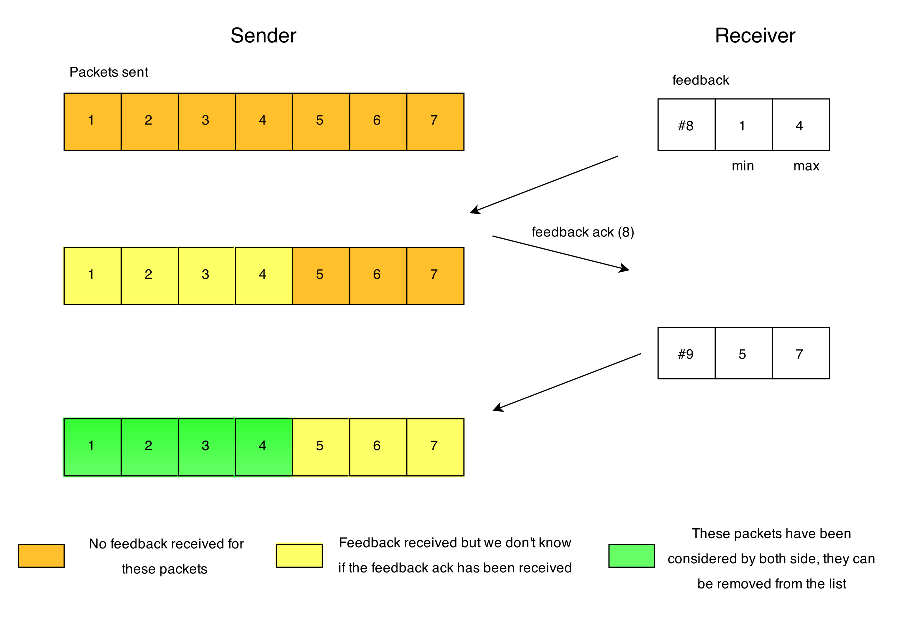
\includegraphics[width=\textwidth]{images/Feedback-implem1.eps}
\caption{How the feedback works in the sender side}
\label{fig:feedback-imp1}
\end{figure}


When a second feedback arrives, everything below the minimum sequence number reported (packets 1 to 4 in this case) can be removed from the list. The reason we can do that is because the feedback packets are cumulative. It would probably become clearer with the second example on Figure \ref{fig:feedback-imp2}. It is exactly the same scenario as before except that the \texttt{FeedbackAck} is lost. Therefore, on the next feedback, the receiver will report all the statistics from the beginning. In consequence, the sender will have to wait one more feedback to shrink the list.

\begin{figure}[!ht]
\centering
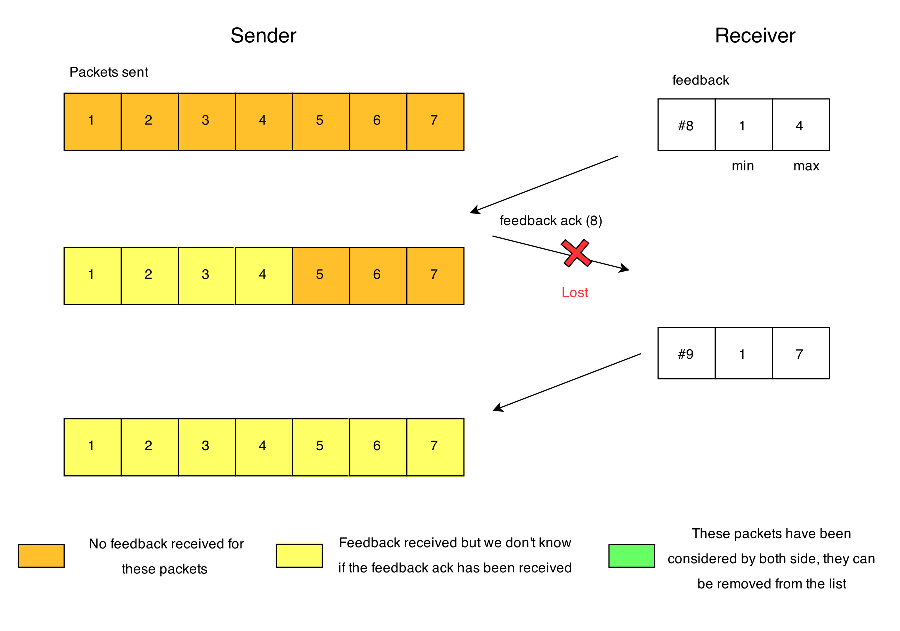
\includegraphics[width=\textwidth]{images/Feedback-implem2.eps}
\caption{How the feedback works in the sender side with losses}
\label{fig:feedback-imp2}
\end{figure}

Note that in our example the sequence number are sequential. It is not a requirement since in practice packets will be sent on different paths and therefore some gaps may be present between sequence numbers on a particular path. Nevertheless will still need the sequence number to be strictly increasing over time for the max-min mechanism to work well. This is guaranteed by DTLS and even if we reach the maximum sequence number allowed, the handshake must first be repeated according to \cite{RFC5246}.

The loss rate is computed every time we received a feedback on the range [min,max] carried by this feedback. This will sometimes cause to compute the loss rate on overlapping sets of packets. This is the case with the scenario presented on figure \ref{fig:feedback-imp2}: we first compute the loss rate on the packets 1 to 4 and then a second time on the packets 1 to 7. As stated in the design part, the loss rate is only an estimation of the real loss rate. However in practice, our system estimates quite accurately the real loss rate (see Section \ref{sec:perfs} for more details). In addition, as recommended in Section \ref{sec:design-loss-rate}, we use an exponential average to consider new loss rates. This prevents short term statistics to impact too heavily the global loss rate of the flow.

\subsection{Receiver Side}

\subsubsection{Structure in Memory}

As for the sender statistics, every flow has too keep some information in memory to monitor the quality of the link. The C structure used is presented on Figure \ref{lst:receiver-stats}. The biggest difference with the sender is the size of the structure which is constant here. Indeed, we don't need to remember every packet received but instead only the minimum and maximum sequence number received so far.

\begin{lstlisting}[caption=Receiver structure to store statistics, label=lst:receiver-stats]
typedef struct MPDTLS_RECEIVER_STATS {
  /* information gathered since the last feedback */
  uint64_t nbr_packets_received;   /* number of packets received */
  uint     min_seq;                /* minimum sequence number */
  uint     max_seq;                /* maximum sequence number  */
  
  /* same information as before but transmitted */
  uint64_t nbr_packets_received_cache;
  uint     min_seq_cache;
  uint     max_seq_cache;
  
  uint64_t backward_delay; /* average backward delay (ms) */
  int      threshold;      /* after how many packets must we send a feedback */
  uint     last_feedback;  /* sequence number of the last feedback we sent */
} MPDTLS_RECEIVER_STATS;
\end{lstlisting}

\subsubsection{Giving feedback}

The way feedback is handled on the receiver side is way more simple than on the sender's. Indeed, we just need to support cumulative feedback. Figure \ref{fig:feedback-imp3} presents the same scenario of Figure \ref{fig:feedback-imp2} but this time on the receiver side. The feedback ack being lost, packets 1 to 4 have not been removed. Indeed, the receiver cannot make the distinction between the loss of the original feedback and the one of the feedback ack.

\begin{figure}[!ht]
\centering
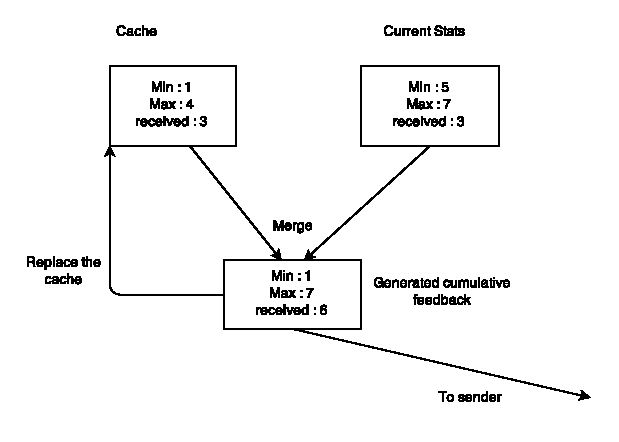
\includegraphics[width=\textwidth]{images/Feedback-implem3.eps}
\caption{How the feedback is generated on the receiver side}
\label{fig:feedback-imp3}
\end{figure}

What we have called the "cache" will aggregate all previous feedback. When the threshold is reached and the receiver has to send feedback, he will first merge the current statistics with the cache to generate the cumulative feedback. The latter is sent to the sender (on the same flow) and the sequence number is remembered in the \texttt{last\_feedback} variable of Listing \ref{lst:receiver-stats}. Then the cache is replaced by this new generated feedback.


\subsubsection{Processing feedback ack}

When a feedback ack is received, the receiver must check if the sequence number corresponds to the last feedback sent. IF they match then the cache is emptied and we are in a situation similar to the one depicted on Figure \ref{fig:feedback-imp1}. The feedback ack carry the sequence number 8 which matches the latest feedback sent thus the cache containing packets 1 to 4 is emptied. Therefore the next feedback will report statistics on packets 5 to 7 only.

If the feedback ack does not contain the sequence number of the latest feedback sent we simply discard it. This kind of situations may be encountered if we have interleaving. 


\subsubsection{Computing backward delay}

The backward delay is computed thanks to regular heartbeat messages going from the sender to the receiver. These messages must transport a timestamp so we have defined a new type of heartbeat called \texttt{HEARTBEAT\_TIMESTAMP}. It allows us to differentiate this kind of message at the record layer stage and perform a different treatment than on standard \texttt{HEARTBEAT\_REQUEST}. 

To get the current time of a system, we use the \texttt{gettimeofday()} function with a \texttt{timeval} structure. It gives a microsecond precision but we actually decided to consider only the milliseconds. After some tests, we have seen that microseconds are not needed because you already loose almost 0.5 ms to do operations on the packet itself (encryption, authentication). From our point of view, milliseconds are enough to capture the network characteristics. If they are two links we cannot differentiate at the millisecond level then we can just consider them as of equal speed (i.e. you will not have a significant enough gain to treat them differently). Of course this could be adapted easily if we have a real interest for such a precision and if network components become much faster.

When the receiver treats a \texttt{HEARTBEAT\_TIMESTAMP}, he computes the absolute value of the difference between his current time and the one contained in the message. This will give the backward delay with the clock desynchronization term. The receiver will add these delays and keep in memory the exponential average (variable \texttt{backward\_delay} of Listing \ref{lst:receiver-stats}). Every time he sends a feedback, he includes his estimation of the backward delay which gives the sender his forward delay.



